\documentclass{standalone}
\usepackage{tikz}
\usetikzlibrary{patterns, positioning}
\usepackage[sfdefault]{ClearSans} %% option 'sfdefault' activates Clear Sans as the default text font
\usepackage[T1]{fontenc}

\begin{document}
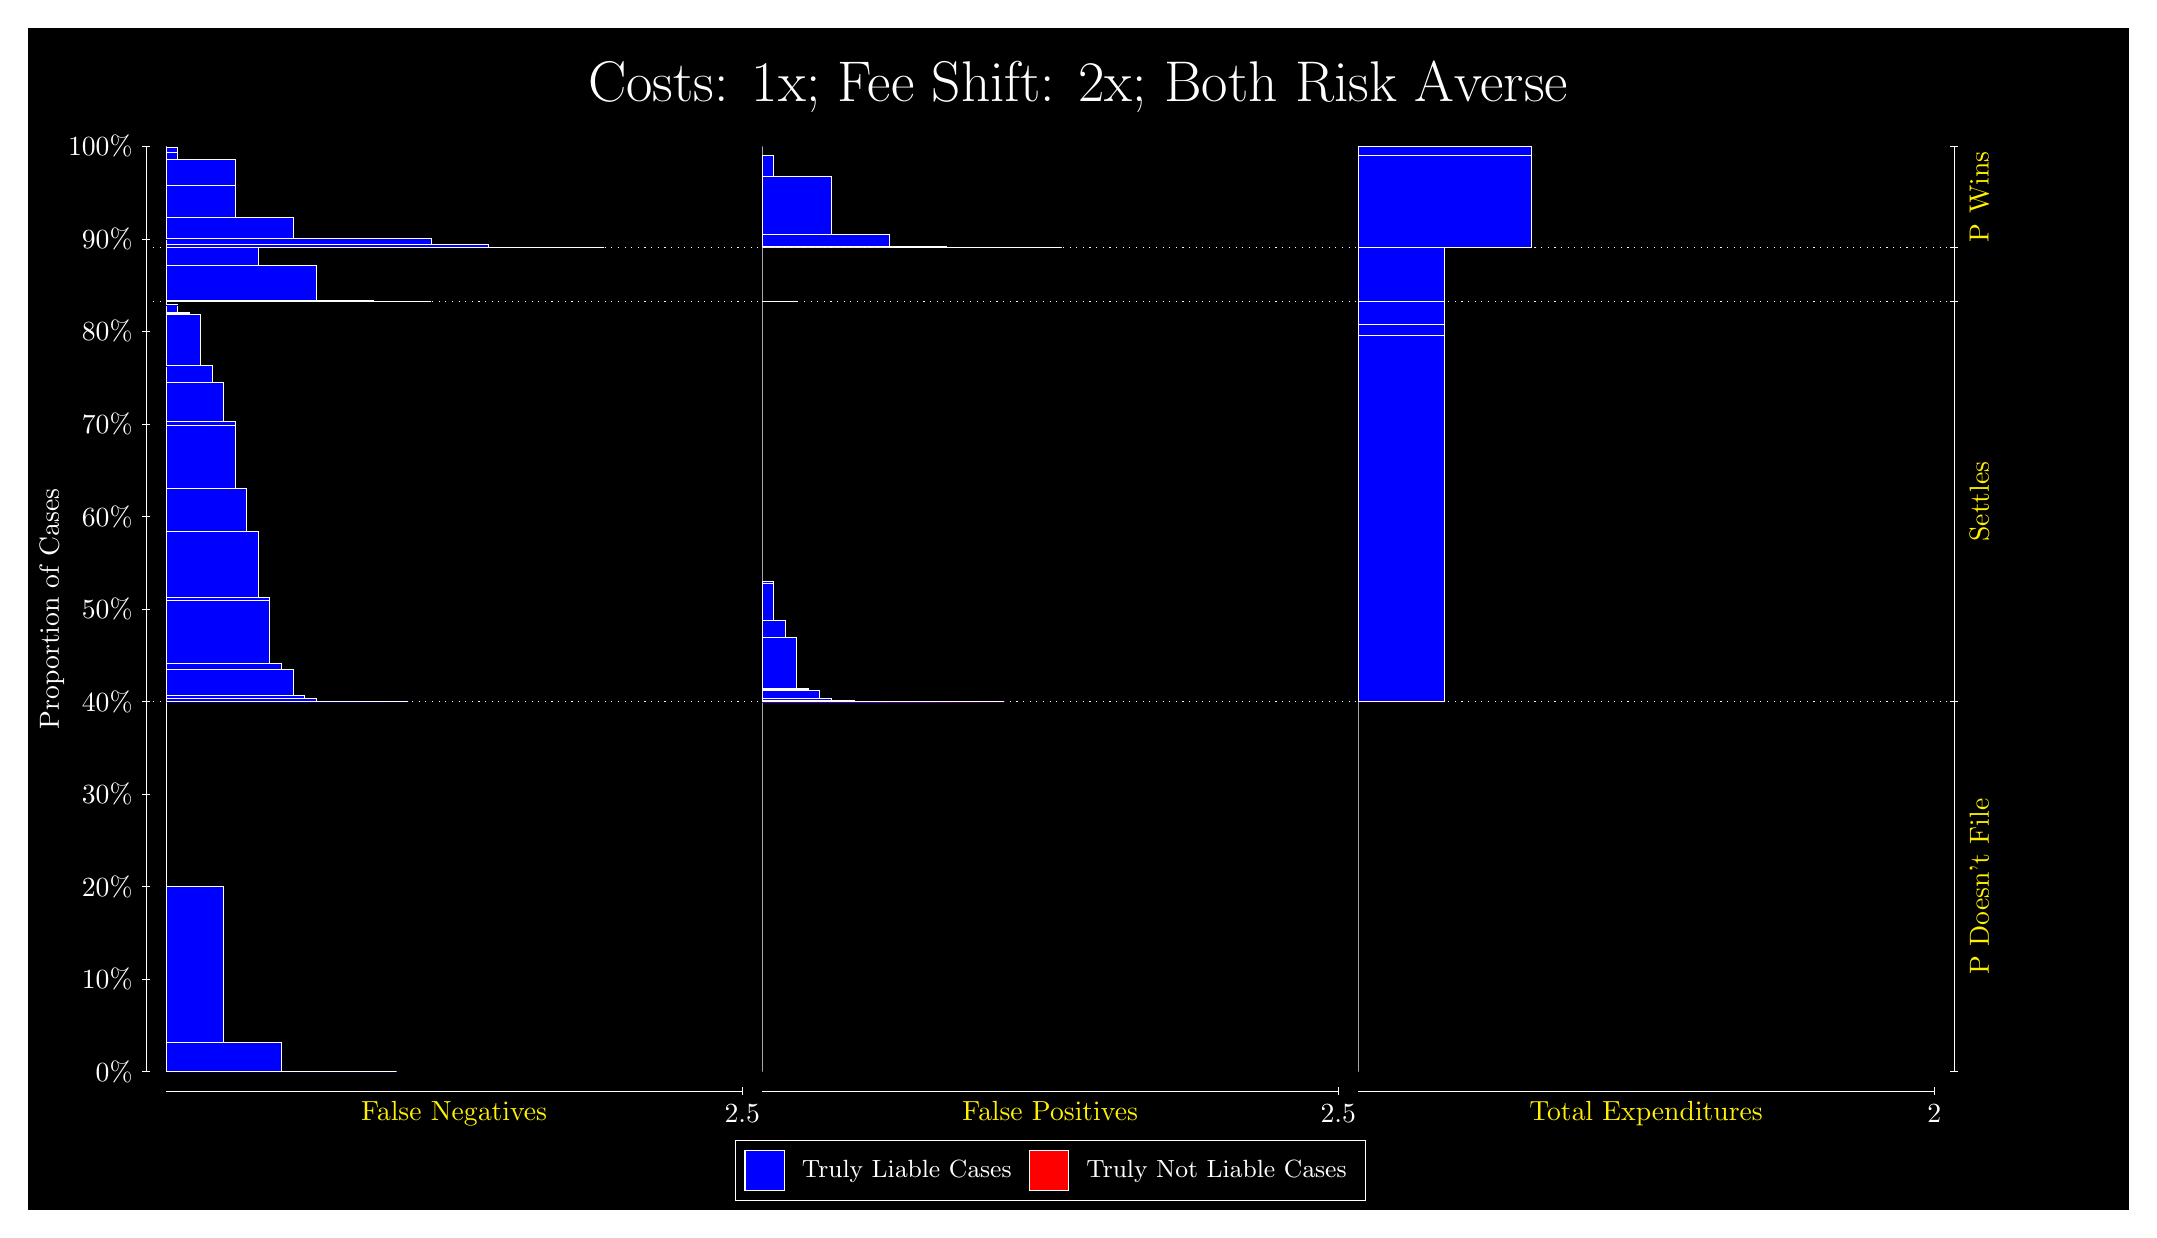
\begin{tikzpicture}
\draw[fill=black] (0,0) rectangle (26.667,15);
\draw[text=white] (0,13.5) rectangle (26.667,15) node[midway] {\huge Costs: 1x; Fee Shift: 2x; Both Risk Averse};
\draw[white, very thin] (1.5,1.75) -- (1.5,13.5);
\node[rotate=90, text=white, anchor=center] at (0.3, 7.625) {Proportion of Cases};
\draw[white, very thin] (1.45,1.75) -- (1.55,1.75);
\node[text=white, anchor=east] at (1.45, 1.75) {0\%};
\draw[white, very thin] (1.45,2.925) -- (1.55,2.925);
\node[text=white, anchor=east] at (1.45, 2.925) {10\%};
\draw[white, very thin] (1.45,4.1) -- (1.55,4.1);
\node[text=white, anchor=east] at (1.45, 4.1) {20\%};
\draw[white, very thin] (1.45,5.275) -- (1.55,5.275);
\node[text=white, anchor=east] at (1.45, 5.275) {30\%};
\draw[white, very thin] (1.45,6.45) -- (1.55,6.45);
\node[text=white, anchor=east] at (1.45, 6.45) {40\%};
\draw[white, very thin] (1.45,7.625) -- (1.55,7.625);
\node[text=white, anchor=east] at (1.45, 7.625) {50\%};
\draw[white, very thin] (1.45,8.8) -- (1.55,8.8);
\node[text=white, anchor=east] at (1.45, 8.8) {60\%};
\draw[white, very thin] (1.45,9.975) -- (1.55,9.975);
\node[text=white, anchor=east] at (1.45, 9.975) {70\%};
\draw[white, very thin] (1.45,11.15) -- (1.55,11.15);
\node[text=white, anchor=east] at (1.45, 11.15) {80\%};
\draw[white, very thin] (1.45,12.325) -- (1.55,12.325);
\node[text=white, anchor=east] at (1.45, 12.325) {90\%};
\draw[white, very thin] (1.45,13.5) -- (1.55,13.5);
\node[text=white, anchor=east] at (1.45, 13.5) {100\%};

\draw[white, very thin] (24.457,1.75) -- (24.457,13.5);
\draw[white, very thin] (24.407,1.75) -- (24.507,1.75);
\node[anchor=west] at (24.407, 1.75) {};
\draw[white, very thin] (24.407,6.4489) -- (24.507,6.4489);
\node[anchor=west] at (24.407, 6.4489) {};
\draw[white, very thin] (24.407,11.53) -- (24.507,11.53);
\node[anchor=west] at (24.407, 11.53) {};
\draw[white, very thin] (24.407,12.219) -- (24.507,12.219);
\node[anchor=west] at (24.407, 12.219) {};
\draw[white, very thin] (24.407,13.5) -- (24.507,13.5);
\node[anchor=west] at (24.407, 13.5) {};

\draw[white, very thin, fill=blue] (1.75,1.75) rectangle (4.6775,1.75);
\draw[white, very thin, fill=blue] (1.75,1.75) rectangle (3.9457,1.7532);
\draw[white, very thin, fill=blue] (1.75,1.7532) rectangle (3.2138,2.126);
\draw[white, very thin, fill=blue] (1.75,2.126) rectangle (2.4819,4.1027);
\draw[white, very thin, fill=red] (1.75,4.1027) rectangle (1.75,4.1027);
\draw[white, very thin, fill=blue] (1.75,4.1027) rectangle (1.75,6.4489);
\draw[white, very thin, fill=blue] (1.75,6.4489) rectangle (4.8239,6.4489);
\draw[white, very thin, fill=blue] (1.75,6.4489) rectangle (4.5312,6.4489);
\draw[white, very thin, fill=blue] (1.75,6.4489) rectangle (4.2384,6.449);
\draw[white, very thin, fill=blue] (1.75,6.449) rectangle (4.092,6.4512);
\draw[white, very thin, fill=blue] (1.75,6.4512) rectangle (3.9457,6.4516);
\draw[white, very thin, fill=blue] (1.75,6.4516) rectangle (3.7993,6.4532);
\draw[white, very thin, fill=blue] (1.75,6.4532) rectangle (3.6529,6.4957);
\draw[white, very thin, fill=blue] (1.75,6.4957) rectangle (3.5065,6.524);
\draw[white, very thin, fill=blue] (1.75,6.524) rectangle (3.3602,6.8604);
\draw[white, very thin, fill=blue] (1.75,6.8604) rectangle (3.2138,6.933);
\draw[white, very thin, fill=blue] (1.75,6.933) rectangle (3.0674,7.7402);
\draw[white, very thin, fill=blue] (1.75,7.7402) rectangle (3.0674,7.769);
\draw[white, very thin, fill=blue] (1.75,7.769) rectangle (2.921,8.6104);
\draw[white, very thin, fill=blue] (1.75,8.6104) rectangle (2.7746,9.1587);
\draw[white, very thin, fill=blue] (1.75,9.1587) rectangle (2.6283,9.9555);
\draw[white, very thin, fill=blue] (1.75,9.9555) rectangle (2.6283,10.007);
\draw[white, very thin, fill=blue] (1.75,10.007) rectangle (2.4819,10.503);
\draw[white, very thin, fill=blue] (1.75,10.503) rectangle (2.3355,10.714);
\draw[white, very thin, fill=blue] (1.75,10.714) rectangle (2.3355,10.716);
\draw[white, very thin, fill=blue] (1.75,10.716) rectangle (2.1891,11.367);
\draw[white, very thin, fill=blue] (1.75,11.367) rectangle (2.0428,11.376);
\draw[white, very thin, fill=blue] (1.75,11.376) rectangle (2.0428,11.39);
\draw[white, very thin, fill=blue] (1.75,11.39) rectangle (1.8964,11.489);
\draw[white, very thin, fill=blue] (1.75,11.489) rectangle (1.8964,11.49);
\draw[white, very thin, fill=blue] (1.75,11.49) rectangle (1.75,11.49);
\draw[white, very thin, fill=red] (1.75,11.49) rectangle (1.75,11.49);
\draw[white, very thin, fill=blue] (1.75,11.49) rectangle (1.75,11.53);
\draw[white, very thin, fill=blue] (1.75,11.53) rectangle (5.1167,11.53);
\draw[white, very thin, fill=blue] (1.75,11.53) rectangle (4.3848,11.545);
\draw[white, very thin, fill=blue] (1.75,11.545) rectangle (3.6529,11.988);
\draw[white, very thin, fill=blue] (1.75,11.988) rectangle (2.921,12.216);
\draw[white, very thin, fill=blue] (1.75,12.216) rectangle (2.1891,12.219);
\draw[white, very thin, fill=red] (1.75,12.219) rectangle (1.75,12.219);
\draw[white, very thin, fill=blue] (1.75,12.219) rectangle (7.3123,12.219);
\draw[white, very thin, fill=blue] (1.75,12.219) rectangle (6.5805,12.219);
\draw[white, very thin, fill=blue] (1.75,12.219) rectangle (5.8486,12.25);
\draw[white, very thin, fill=blue] (1.75,12.25) rectangle (5.1167,12.327);
\draw[white, very thin, fill=blue] (1.75,12.327) rectangle (4.8239,12.327);
\draw[white, very thin, fill=blue] (1.75,12.327) rectangle (4.3848,12.328);
\draw[white, very thin, fill=blue] (1.75,12.328) rectangle (4.092,12.33);
\draw[white, very thin, fill=blue] (1.75,12.33) rectangle (3.6529,12.33);
\draw[white, very thin, fill=blue] (1.75,12.33) rectangle (3.3602,12.598);
\draw[white, very thin, fill=blue] (1.75,12.598) rectangle (2.921,12.598);
\draw[white, very thin, fill=blue] (1.75,12.598) rectangle (2.6283,13.011);
\draw[white, very thin, fill=blue] (1.75,13.011) rectangle (2.6283,13.34);
\draw[white, very thin, fill=blue] (1.75,13.34) rectangle (1.8964,13.423);
\draw[white, very thin, fill=blue] (1.75,13.423) rectangle (1.8964,13.493);
\draw[white, very thin, fill=red] (1.75,13.493) rectangle (1.75,13.493);
\draw[white, very thin, fill=blue] (1.75,13.493) rectangle (1.75,13.5);
\draw[white, very thin, fill=red] (9.3189,1.75) rectangle (9.3189,1.75);
\draw[white, very thin, fill=blue] (9.3189,1.75) rectangle (9.3189,6.4489);
\draw[white, very thin, fill=red] (9.3189,6.4489) rectangle (12.393,6.4489);
\draw[white, very thin, fill=blue] (9.3189,6.4489) rectangle (12.393,6.4489);
\draw[white, very thin, fill=red] (9.3189,6.4489) rectangle (12.1,6.4489);
\draw[white, very thin, fill=blue] (9.3189,6.4489) rectangle (12.1,6.4489);
\draw[white, very thin, fill=red] (9.3189,6.4489) rectangle (11.807,6.4489);
\draw[white, very thin, fill=blue] (9.3189,6.4489) rectangle (11.807,6.4489);
\draw[white, very thin, fill=blue] (9.3189,6.4489) rectangle (11.661,6.4489);
\draw[white, very thin, fill=red] (9.3189,6.4489) rectangle (11.515,6.4489);
\draw[white, very thin, fill=blue] (9.3189,6.4489) rectangle (11.515,6.4489);
\draw[white, very thin, fill=blue] (9.3189,6.4489) rectangle (11.368,6.4489);
\draw[white, very thin, fill=red] (9.3189,6.4489) rectangle (11.222,6.4489);
\draw[white, very thin, fill=blue] (9.3189,6.4489) rectangle (11.222,6.4489);
\draw[white, very thin, fill=blue] (9.3189,6.4489) rectangle (11.075,6.4489);
\draw[white, very thin, fill=red] (9.3189,6.4489) rectangle (10.929,6.4489);
\draw[white, very thin, fill=blue] (9.3189,6.4489) rectangle (10.929,6.4489);
\draw[white, very thin, fill=red] (9.3189,6.4489) rectangle (10.929,6.4489);
\draw[white, very thin, fill=blue] (9.3189,6.4489) rectangle (10.929,6.4489);
\draw[white, very thin, fill=blue] (9.3189,6.4489) rectangle (10.783,6.4491);
\draw[white, very thin, fill=blue] (9.3189,6.4491) rectangle (10.636,6.4491);
\draw[white, very thin, fill=red] (9.3189,6.4491) rectangle (10.636,6.4491);
\draw[white, very thin, fill=blue] (9.3189,6.4491) rectangle (10.636,6.4491);
\draw[white, very thin, fill=blue] (9.3189,6.4491) rectangle (10.49,6.4689);
\draw[white, very thin, fill=red] (9.3189,6.4689) rectangle (10.344,6.4689);
\draw[white, very thin, fill=blue] (9.3189,6.4689) rectangle (10.344,6.4698);
\draw[white, very thin, fill=blue] (9.3189,6.4698) rectangle (10.197,6.4894);
\draw[white, very thin, fill=blue] (9.3189,6.4894) rectangle (10.197,6.4895);
\draw[white, very thin, fill=red] (9.3189,6.4895) rectangle (10.051,6.4895);
\draw[white, very thin, fill=blue] (9.3189,6.4895) rectangle (10.051,6.5899);
\draw[white, very thin, fill=blue] (9.3189,6.5899) rectangle (9.9044,6.6039);
\draw[white, very thin, fill=blue] (9.3189,6.6039) rectangle (9.9044,6.6123);
\draw[white, very thin, fill=blue] (9.3189,6.6123) rectangle (9.758,7.2636);
\draw[white, very thin, fill=blue] (9.3189,7.2636) rectangle (9.6116,7.4761);
\draw[white, very thin, fill=blue] (9.3189,7.4761) rectangle (9.4652,7.9527);
\draw[white, very thin, fill=blue] (9.3189,7.9527) rectangle (9.4652,7.9728);
\draw[white, very thin, fill=blue] (9.3189,7.9728) rectangle (9.3189,11.53);
\draw[white, very thin, fill=red] (9.3189,11.53) rectangle (9.758,11.53);
\draw[white, very thin, fill=blue] (9.3189,11.53) rectangle (9.758,11.533);
\draw[white, very thin, fill=blue] (9.3189,11.533) rectangle (9.3189,12.219);
\draw[white, very thin, fill=red] (9.3189,12.219) rectangle (13.125,12.219);
\draw[white, very thin, fill=blue] (9.3189,12.219) rectangle (13.125,12.219);
\draw[white, very thin, fill=red] (9.3189,12.219) rectangle (12.393,12.219);
\draw[white, very thin, fill=blue] (9.3189,12.219) rectangle (12.393,12.219);
\draw[white, very thin, fill=red] (9.3189,12.219) rectangle (11.661,12.219);
\draw[white, very thin, fill=blue] (9.3189,12.219) rectangle (11.661,12.225);
\draw[white, very thin, fill=red] (9.3189,12.225) rectangle (10.929,12.225);
\draw[white, very thin, fill=blue] (9.3189,12.225) rectangle (10.929,12.379);
\draw[white, very thin, fill=blue] (9.3189,12.379) rectangle (10.197,13.121);
\draw[white, very thin, fill=red] (9.3189,13.121) rectangle (9.9044,13.121);
\draw[white, very thin, fill=blue] (9.3189,13.121) rectangle (9.9044,13.121);
\draw[white, very thin, fill=blue] (9.3189,13.121) rectangle (9.4652,13.389);
\draw[white, very thin, fill=red] (9.3189,13.389) rectangle (9.3189,13.389);
\draw[white, very thin, fill=blue] (9.3189,13.389) rectangle (9.3189,13.5);
\draw[white, very thin, fill=red] (16.888,1.75) rectangle (16.888,1.75);
\draw[white, very thin, fill=blue] (16.888,1.75) rectangle (16.888,6.4489);
\draw[white, very thin, fill=red] (16.888,6.4489) rectangle (17.986,6.4489);
\draw[white, very thin, fill=blue] (16.888,6.4489) rectangle (17.986,11.105);
\draw[white, very thin, fill=red] (16.888,11.105) rectangle (17.986,11.105);
\draw[white, very thin, fill=blue] (16.888,11.105) rectangle (17.986,11.239);
\draw[white, very thin, fill=red] (16.888,11.239) rectangle (17.986,11.239);
\draw[white, very thin, fill=blue] (16.888,11.239) rectangle (17.986,11.53);
\draw[white, very thin, fill=red] (16.888,11.53) rectangle (17.986,11.53);
\draw[white, very thin, fill=blue] (16.888,11.53) rectangle (17.986,12.219);
\draw[white, very thin, fill=red] (16.888,12.219) rectangle (19.083,12.219);
\draw[white, very thin, fill=blue] (16.888,12.219) rectangle (19.083,13.39);
\draw[white, very thin, fill=red] (16.888,13.39) rectangle (19.083,13.39);
\draw[white, very thin, fill=blue] (16.888,13.39) rectangle (19.083,13.5);
\draw[white, dotted] (1.5,6.4489) -- (24.457,6.4489);
\draw[white, dotted] (1.5,11.53) -- (24.457,11.53);
\draw[white, dotted] (1.5,12.219) -- (24.457,12.219);
\draw[white, very thin] (1.75,1.5) -- (9.0689,1.5);
\node[text=yellow, anchor=north] at (5.4094, 1.5) {False Negatives};
\draw[white, very thin] (9.0689,1.45) -- (9.0689,1.55);
\node[text=white, anchor=north] at (9.0689, 1.45) {2.5};

\draw[white, very thin] (9.3189,1.5) -- (16.638,1.5);
\node[text=yellow, anchor=north] at (12.978, 1.5) {False Positives};
\draw[white, very thin] (16.638,1.45) -- (16.638,1.55);
\node[text=white, anchor=north] at (16.638, 1.45) {2.5};

\draw[white, very thin] (16.888,1.5) -- (24.207,1.5);
\node[text=yellow, anchor=north] at (20.547, 1.5) {Total Expenditures};
\draw[white, very thin] (24.207,1.45) -- (24.207,1.55);
\node[text=white, anchor=north] at (24.207, 1.45) {2};

\node[text=yellow, centered, rotate=90] at (24.777, 4.0995) {P Doesn't File};
\node[text=yellow, centered, rotate=90] at (24.777, 8.9897) {Settles};

\node[text=yellow, centered, rotate=90] at (24.777, 12.859) {P Wins};

\draw (12.978300999999998,1.5) node[draw=none] (baseCoordinate) {};
\begin{scope}[align=center]
        \matrix[scale=0.5, draw=white, below=0.5cm of baseCoordinate, nodes={draw}, column sep=0.1cm]{
            \node[rectangle, draw, minimum width=0.5cm, minimum height=0.5cm, fill=blue] {}; &
            \node[draw=none, font=\small, text=white] (B) {Truly Liable Cases}; &
            \node[rectangle, draw, minimum width=0.5cm, minimum height=0.5cm, fill=red] {}; &
            \node[draw=none, font=\small, text=white] (B) {Truly Not Liable Cases}; \\
            };
\end{scope}

\end{tikzpicture}
\end{document}